\section{Adding non-determinism and overspecification} \label{sec:algorithm}

Refinement algorithms for GRE are based on the following basic idea: given a 
scene $S$, the objects appearing in $S$ are successively classified according
to their properties into finer and finer classes. A description (in some formal language $\mathcal{L}$) of each 
class is computed every time a class is refined. The procedure always stops when the 
set of classes stabilizes, i.e., no further refinement is possible with the information 
available in the scene\footnote{Of course, if we are only interested in a referring expression for 
a given target we can stop the procedure as soon as the target is the only element of some of the classes.}.  If the target element is in a singleton class, then the formal description of that class is a referring expression; otherwise the 
target cannot be unequivocally described (in $\mathcal{L}$).  

In this section we present a modification of the algorithm in~\cite{arec2:2008:Areces} where the fixed order of properties in the 
input scene is replaced by a finite probability distribution. Required changes
are fairly straightforward (see Figures~\ref{fig:algo1} and~\ref{fig:algo3}), but 
the behavior of the resulting algorithm is strikingly changed. To start with, the 
algorithm is now non-deterministic: two runs of the algorithm with the same 
input might result in different REs for objects in the scene.

In order to understand how the algorithm works, and differences with the original proposal, we need first to introduce some 
basic notions. The input to the algorithm will be a relational model $\mathcal{M} = \tup{\Delta, \interp{\cdot}}$,
where $\Delta$ is the non-empty domain of objects in the scene, and $\interp{\cdot}$ is an 
interpretation function that assigns to all properties in the scene its intended extension.  For example, 
the scene shown in Figure~\ref{GRE3D7-stimulus} could be represented by the model $\gM=\tup{\Delta,\interp{\cdot}}$ shown in Figure~\ref{GRE3D7-stimulus-graph}; where $\Delta = \{e_1,\ldots,e_7\}$, and $\interp{\emph{green}}$, for example, is $\{e_3,e_4,e_6\}$.

\newcommand{\nBlue}{\mathit{blue}\xspace}
\newcommand{\nGreen}{\mathit{green}\xspace}
\newcommand{\nSmall}{\mathit{small}\xspace}
\newcommand{\nBig}{\mathit{big}\xspace}
\newcommand{\nBall}{\mathit{ball}\xspace}
\newcommand{\nCube}{\mathit{cube}\xspace}
\newcommand{\nOntop}{\mathit{ontop}\xspace}
\newcommand{\nTop}{\mathit{top}\xspace}
\newcommand{\nBelow}{\mathit{below}\xspace}
\newcommand{\nRightof}{\mathit{rightof}\xspace}
\newcommand{\nLeftof}{\mathit{leftof}\xspace}
\newcommand{\nLeft}{\mathit{left}\xspace}

\begin{figure}[ht]
\begin{minipage}[b]{0.45\linewidth}
\centering
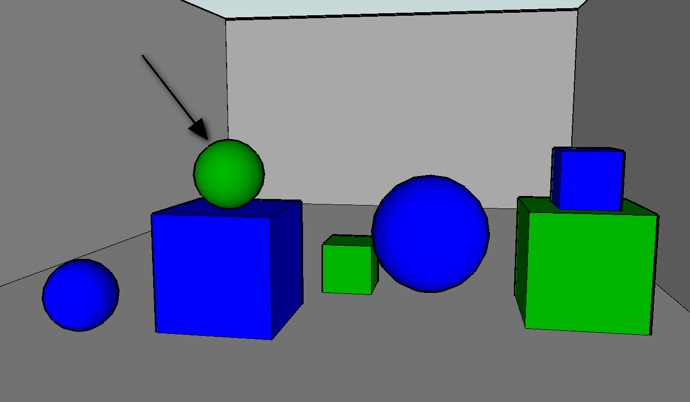
\includegraphics[width=\textwidth]{images/3.jpg}
\vspace*{.15cm}
\caption{Input scene}
\label{GRE3D7-stimulus}
\end{minipage}
\hspace*{-0.35cm}
\begin{minipage}[b]{0.6\linewidth}
\centering
\begin{tikzpicture}
  [
    n/.style={circle,fill,draw,inner sep=3pt,node distance=1.4cm},
    aArrow/.style={->, >=stealth, semithick, shorten <= 2pt, shorten >= 2pt},
  ]
 \node[n,label=above:$e_1$,label=below:{
    \relsize{-1}$\begin{array}{c}
      \nLeft\\[-2pt]
      \nSmall\\[-2pt] 
      \nBlue \\[-2pt] 
      \nBall\end{array}$}] (a) {};

 \node[n,label=above:$e_2$,label=below:{
    \relsize{-1}$\begin{array}{c}
      \nLeft\\[-2pt]
      \nBig\\[-2pt] 
      \nBlue\\[-2pt] 
      \nCube\end{array}$}, right of=a] (b) {};

 \node[n,label=below:$e_3$,label=above:{
    \relsize{-1}$\begin{array}{c}
      \nTop\\[-2pt]
      \nLeft\\[-2pt]
      \nSmall\\[-2pt] 
      \nGreen\\[-2pt] 
      \nBall\end{array}$}, above of=b] (c) {};

 \node[n,label=above:$e_4$,label=below:{
    \relsize{-1}$\begin{array}{c}
      \nSmall\\[-2pt] 
      \nGreen\\[-2pt] 
      \nCube\end{array}$}, right of=b] (d) {};

 \node[n,label=above:$e_5$,label=below:{
    \relsize{-1}$\begin{array}{c}
      \nBig\\[-2pt] 
      \nBlue\\[-2pt] 
      \nBall\end{array}$}, right of=d] (e) {};

 \node[n,label=above:$e_6$,label=below:{
    \relsize{-1}$\begin{array}{c}
      \nBig\\[-2pt] 
      \nGreen\\[-2pt] 
      \nCube\end{array}$}, right of=e] (f) {};

 \node[n,label=below:$e_7$,label=above:{
    \relsize{-1}$\begin{array}{c}
      \nTop\\[-2pt]
      \nSmall\\[-2pt] 
      \nBlue\\[-2pt] 
      \nCube\end{array}$}, above of=f] (g) {};

 \draw [aArrow,bend right=90] (b) to node[auto,swap]{\relsize{-1}$\nBelow$} (c);
 \draw [aArrow,bend right=90] (c) to node[auto,swap]{\relsize{-1}$\nOntop$} (b);

 \draw [aArrow,bend right=30] (d) to node[auto,swap]{\relsize{-1}$\nLeftof$} (e);
 \draw [aArrow,bend right=30] (e) to node[auto,swap]{\relsize{-1}$\nRightof$} (d);

 \draw [aArrow,bend right=90] (f) to node[auto,swap]{\relsize{-1}$\nBelow$} (g);
 \draw [aArrow,bend right=90] (g) to node[auto,swap]{\relsize{-1}$\nOntop$} (f);

 \draw[dotted] (-.4,-1.4) rectangle (7.1,3.1);

 \end{tikzpicture}
\caption{Scene as a relational model}
\label{GRE3D7-stimulus-graph}
\end{minipage}
\end{figure}

It is clear that a scene can be encoded in different ways as a relational model (for example, we could argue that $e_1$ is also \emph{leftof} $e_2$, and so on). The algorithm assumes that these issues have been resolved and that the model encodes a suitable representation of the scene we want to describe. Moreover, we will assume that all relations are \emph{binary}. We will not consider relations of arity greater than two (relations of higher arity can be encoded as binary relations via reification, if necessary), and unary
properties can be encoded as binary relations including one additional `dummy' element in the model (e.g., we encode the fact that $e_1$ is \emph{blue} saying that it is related to the dummy element by the \emph{blue} binary relation).

On termination, the algorithm computes what are called the $\mathcal{L}$-similarity classes of the input model $\gM$. Intuitively, if two elements in the model belong to the same $\mathcal{L}$-similarity class, then $\mathcal{L}$ is not expressive enough to tell them appart (i.e, no formula in $\mathcal{L}$ can distinguish them). 

In what follows, we will use formulas of the $\el$ description logic language~\cite{baad:desc03} to describe refinement classes.  As discussed in~\cite{arec2:2008:Areces}, this language is suitable for conjunctive relational RE, which are ones we will find in the corpora used for our evaluation\footnote{Notice, though, that the particular formal language used is independent of the main algorithm, and different add$_{\mathcal{L}}$(R,$\varphi$,\RE) functions can be used depending on the language involved.}. For a detailed description of $\el$, we refer to~\cite{baad:desc03}.  For this paper, we only need to know that the interpretation of the formula $\psi \sqcap \exists$R.$\varphi$ is the set of all elements that satisfy $\psi$ and that are related by relation R to some element that satisfy $\varphi$. For example, the interpretation of the formula \emph{ball} $\sqcap \exists$\emph{leftof}.\emph{cube} is the set of all balls that are on the left of some cube.  

We are now ready to describe Algorithms~\ref{algo:bisim-l} and~\ref{algo:bisim-add-el-over}. Algorithm~\ref{algo:bisim-l} takes as input a model $\gM$ and a list Rs of pairs (R,R.\puse) that links each relation R to some probability of use R.\puse. I.e., if $\REL$ is the set of all relation symbols in the model (i.e., the \emph{signature} of the model) then Rs $\in (\REL \times [0,1])^*$. Moreover, we assume Rs to be ordered by R.\puse. 

\begin{figure}[t]
\small
\centering
\begin{algorithm}[H]
\dontprintsemicolon
\caption{Computing $\mathcal{L}$-similarity classes}\label{algo:bisim-l}
\KwIn{\footnotesize A model $\gM$ and a list Rs $\in (\REL \times [0,1])^*$
 of relation symbols with their \puse\ values, ordered by \puse}
\KwOut{\footnotesize A set of formulas \RE such that
$\{\interp{\varphi} \mid \varphi \in \RE\}$ is the set of
$\mathcal{L}$-similarity classes of $\gM$}

$\RE \leftarrow \{\top\}$\tcp*[f]{\footnotesize the most general description $\top$ applies to all elements in the scene}

\For{\em (R,R.\puse) $\in$ Rs}{
	R.\randomuse = Random(0,1)\tcp*[f]{\footnotesize R.\randomuse is the probability of using R} \;
        R.\incuse = (1 $-$ R.\puse) / MaxIterations\tcp*[f]{\footnotesize R.\puse\ are incremented by R.\incuse in each loop}
}

\Repeat{\em $\forall$((R,R.\puse) $\in$ Rs).(R.\puse $\ge$ 1)\tcp*[f]{\footnotesize R.\puse\ are incremented until they reach 1}}{
  \While(\tcp*[f]{\footnotesize while some class has at least two elements}){\em $\exists (\varphi \in$ \RE)$.(|\interp{\varphi}|>1)$}{
      \RE' $\leftarrow$ \RE \tcp*[f]{\footnotesize make a copy for future comparison} \;
      \For{\em (R, R.\puse) $\in$ Rs}{
          \If(\tcp*[f]{\footnotesize R will be used in the expression}){\em R.\randomuse $\le$ R.\puse}{
              \For{\em $\varphi \in$ \RE}{
                  add$_\mathcal{L}$(R, $\varphi$, \RE)\tcp*[f]{\footnotesize refine all classes using R}}
                  }\;
              \If(\tcp*[f]{\footnotesize the classification has changed}){\em \RE $\not =$ \RE'}{exit\tcp*[f]{\footnotesize exit for-loop to try again highest R.\puse}}
              }
     \If(\tcp*[f]{\footnotesize the classification has stabilized}){\em \RE $=$ \RE'}{exit\tcp*[f]{\footnotesize exit while-loop to increase R.\puse}}
  }
  \For{\em (R,R.\puse) $\in$ Rs}{
    R.\puse $\leftarrow$ R.\puse $+$ R.\incuse\tcp*[f]{\footnotesize increase R.\puse}
  }
}
\end{algorithm}
\vspace*{-.5cm}\caption{Main algorithm, dealing with probabilities}\label{fig:algo1}
\end{figure}

The set $\RE$ will contain the formal description of the refinement classes and it is initialized by the most general description $\top$.  
For each R, we first compute R.\randomuse, a random number in [0,1].  If R.\randomuse $\le$ R.\puse\ then we will use R to refine the set of classes.  The value of R.\puse\ will be incremented by $R.\incuse$ in each main loop, to ensure that all relations are, at some point, considered by the algorithm.  This ensures that a referring expression will be found if it exist; but gives higher probability to expressions using relations with a high R.\puse. 
 
While $\RE$ contains descriptions that can be refined (i.e., classes with at least two elements) we will call the refinement function add$_\mathcal{L}$(R,$\varphi$,$\RE$) successively with each relation in Rs. A change in one of the classes, can trigger changes in others. For that reason, if $\RE$ changes, we exit the for-loop to start again with the relations of higher R.\puse. If the after trying to refine the set with all relations in Rs, the set $\RE$ has not changed, the we have reach a stable state (i.e., the classes described in $\RE$ cannot be further refined, using the current R.\puse\ values). We will then increment all the R.\puse\ values and start the procedure again. 

\begin{figure}[t]
\small
\centering
\begin{algorithm}[H]
\dontprintsemicolon
\caption{add$_\el$(R, $\varphi$, \RE)} \label{algo:bisim-add-el-over}

\eIf(\tcp*[f]{\footnotesize are we in the first loop?}){\em FirstLoop?}{
    Informative $\leftarrow$ $\top$ \tcp*[f]{\footnotesize allow overspecification}}{
    Informative $\leftarrow$ $\interp{\psi \sqcap \exists \mbox{\em R}.\varphi} \neq \interp{\psi}$ \tcp*[f]{\footnotesize informative: smaller than the original?}}
\For{\em $\psi \in$ \RE with $|\interp{\psi}| > 1$}{
  \If{\em $\psi \sqcap \exists$R.$\varphi$ is not subsumed in \RE\ {\bf and} \tcp*[f]{\footnotesize non-redundant: can't be obtained form \RE?}\\
    \em \ \ \ $\interp{\psi \sqcap \exists \mbox{\em R}.\varphi} \neq \emptyset$ {\bf and} \tcp*[f]{\footnotesize non-trivial: has elements?}\\
     \ \ \  \emph{Informative}}{
    add $\psi \sqcap \exists \mbox{R}.\varphi$ to $\RE$ \tcp*[f]{\footnotesize add the new class to the classification} \;
    remove subsumed formulas from $\RE$ \tcp*[f]{\footnotesize remove redundant classes}
  }
}
\end{algorithm}
\vspace*{-.5cm}\caption{Refinement function with overspecification for the \el-language}\label{fig:algo3}
\end{figure}


Algorithm~\ref{algo:bisim-add-el-over} almost coincides with the one described in~\cite{arec2:2008:Areces}.  In the for loop it will refine each descriptions in $\RE$ using the relation R and the other descriptions already in $\RE$, under certain conditions. The new description should be \emph{non-redundant} (the new  class cannot be obtained as the union of classes already represented in $\RE$), \emph{non-trivial} (the new class is not empty), and \emph{informative} (the new class should not coincide with the original class).  If all this conditions are met, the new description is added to $\RE$, and redundant descriptions possible created by the addition of the new description are eliminated. The if else at begining of the algorithm if for do overspecification only in the first loop of the main algorithm.   

%Suppose fixed an input model $\gM$ and values for Rs, and fix also some target element $t$.  Assume also that $t$ indeed has an $\el$-referring expression.  Upon termination, Algorithm~\ref{fig:algo1} will compute an $\el$ formula $\varphi$ such that $\interp{\varphi} = \{t\}$, but $\varphi$ might be different in each run of the algorithm (even though $\gM$ and Rs are fixed).  If we repeat this experiment a statistically significant number of times, we can define an estimate of the probability distribution of the REs generated by the algorithm for $t$, given $\gM$ and Rs. In Section~\ref{sec:evaluation} we will show that given a corpus of REs for $\gM$, it is possible to define R.\puse\ values so that this probability distribution matches with good accuracy the probability distribution of REs found in the corpus.  

